\subsection{System block diagram}
\label{sec:des-system}
Figure~\ref{fig:des-hardware-system} groups the hardware into five parts. External power (1) supplies the ODROID and motor drivers. External interfaces (2) provide page restraint, camera images and operator access. Stepper control (3) converts GPIO commands into winding currents. The belt-driven gantry (4) moves the pen in $x$ and $y$. The pen mechanism (5) switches contact with the page and reports its state. Table~\ref{tab:des-pin-map} in the appendix gives the individual connections.

\begin{figure}[H]\centering
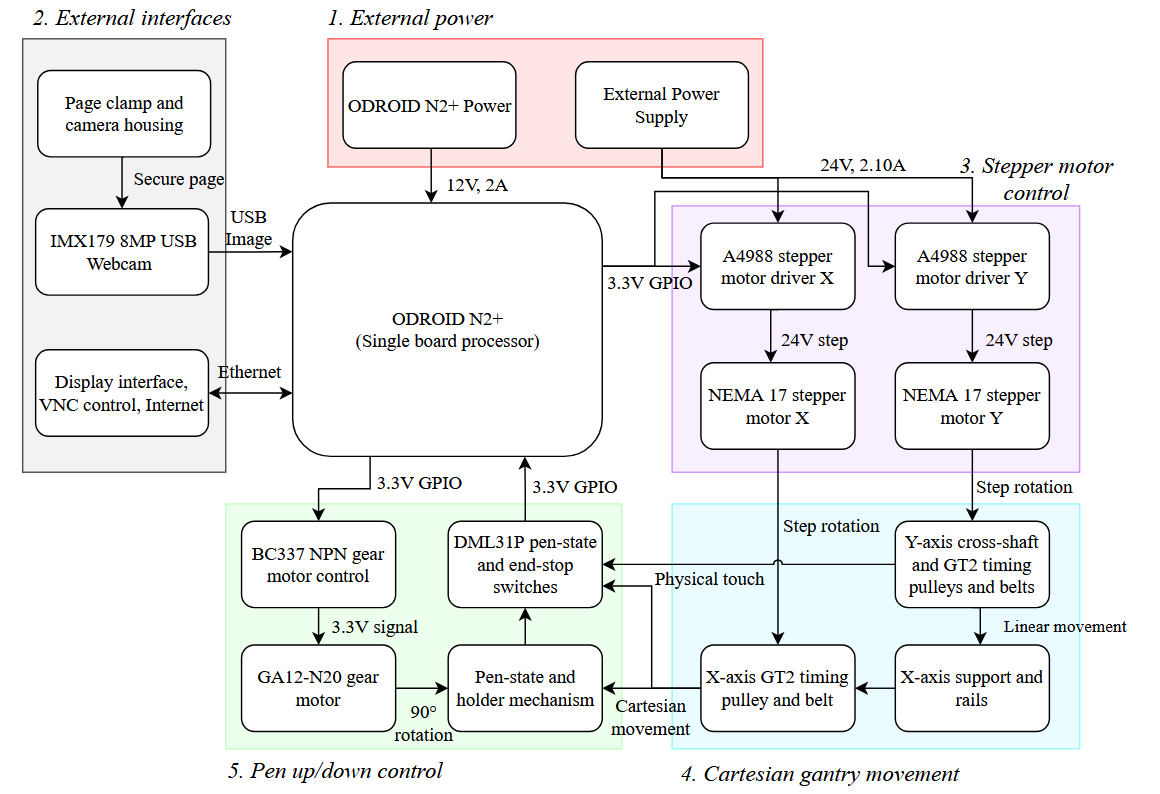
\includegraphics[width=0.96\linewidth]{Evidence/user_hardware_diagram_input.png}
\caption{Hardware system block diagram.}
\label{fig:des-hardware-system}
\end{figure}
\FloatBarrier

Figure~\ref{fig:des-processing-system} shows four software groups. Segmentation (1) conditions a page and returns line crops. Reproduction (2) assembles the selected profile into trajectories and G-code, then executes the path after calibration. Training (3) uses labelled crops to fit the text or writer model and builds stored glyph profiles from labelled handwriting. Classification (4) recognises text or identifies the writer, applying stroke normalisation before writer inference. The diagram groups these functions, while their data dependencies and separate training stages are detailed below.

\begin{figure}[H]\centering
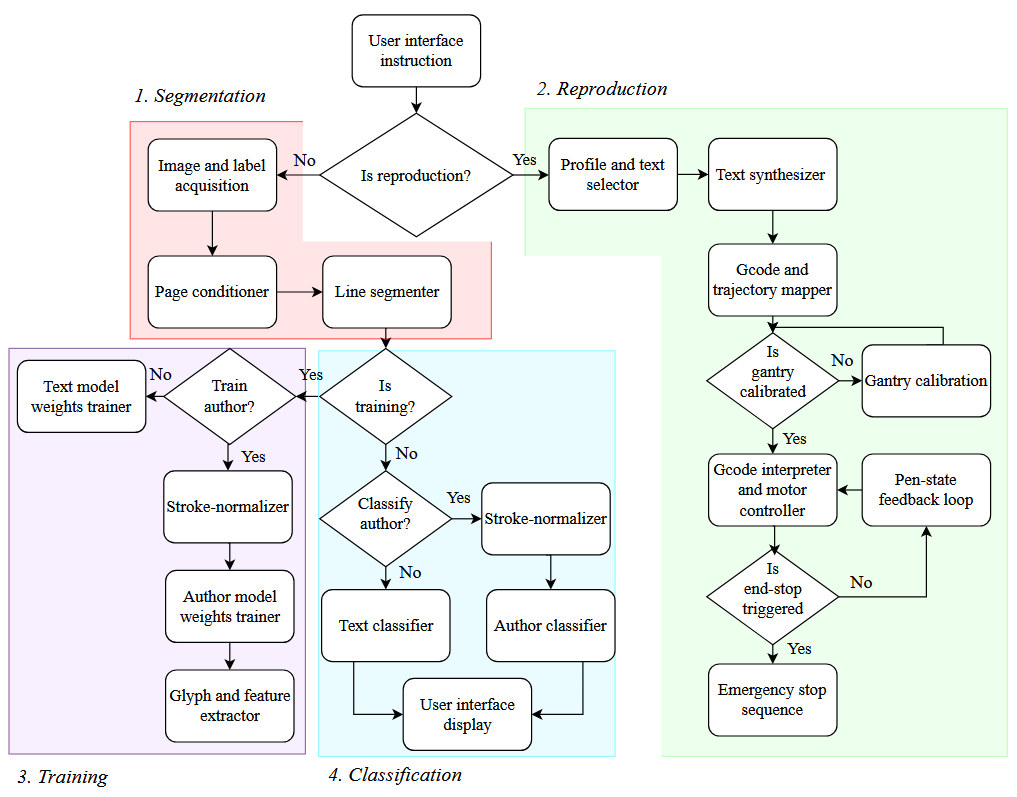
\includegraphics[width=0.98\linewidth]{Evidence/user_software_diagram_input.png}
\caption{Software system block diagram.}
\label{fig:des-processing-system}
\end{figure}

